\section{Programovatelné a neprogramovatelné logické obvody}

\subsection{PLD}
Programovatelný logický obvod je elektronická součástka, která je používána pro vytváření uživatelsky nastavitelných číslicových obvodů. Na rozdíl od hradel, registrů a jiných číslicových obvodů (které mají z výroby pevně danou funkci) musí být PLD před použitím nejprve naprogramováno.

\subsubsection{Rozdělení}
\paragraph{PLA}
PLA je zkratka pro Programovatelné logické pole který představuje booleovskou funkci ve formě SOP (Sum of Products). PLA obsahuje NOT, AND a OR branky vyrobené na čipu. V PLA jsou programovatelná připojení k AND a OR polím. PLA je ve srovnání s PAL považována za nákladnější a složitější.
\begin{figure}[h]
\centering
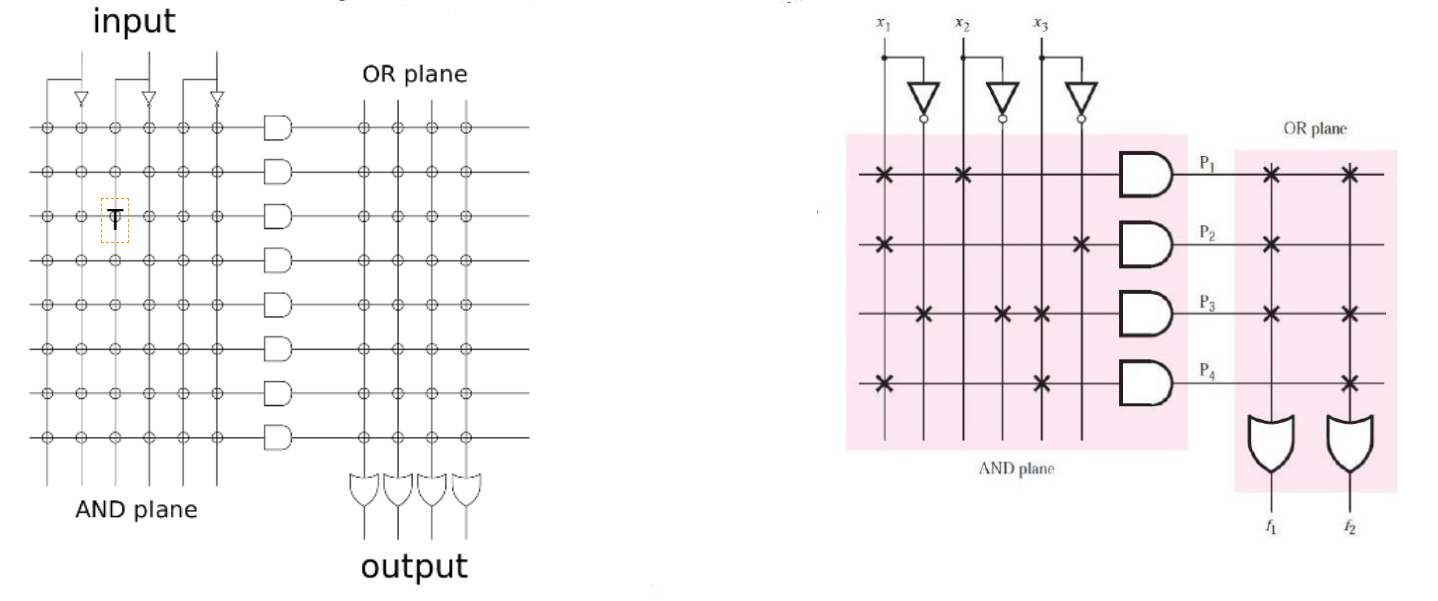
\includegraphics[scale=0.4]{sections/3_pld_npld/images/PLA.png}
\end{figure}

\paragraph{PAL}
Funguje podobně jako PLA. PAL na rozdíl od PLA používá programovatelné AND, ale pevné OR brány.
\begin{figure}[h]
\centering
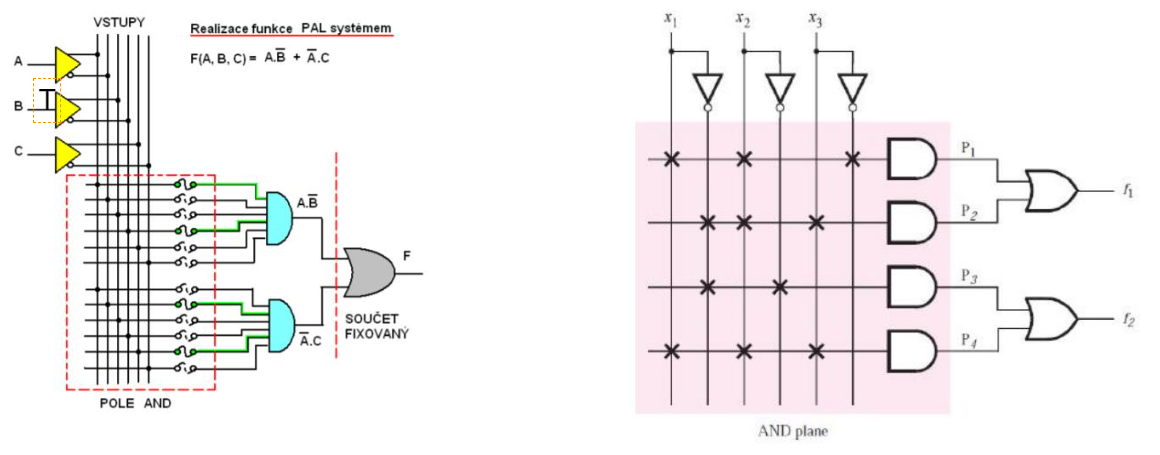
\includegraphics[scale=0.5]{sections/3_pld_npld/images/PAL.png}
\end{figure}

\vspace{25mm}
\paragraph{GAL}
Vylepšená verze PAL, má i stejně vlastnosti a parametry, ale může být přeprogramováno. Typycky také obsahují klopné obvody umožnující sekvenční logiku.

\paragraph{CPLD}
Na obvody CPLD (komplexní programovatelné logické obvody) se můžeme dívat jako na spojení více obvodů GAL nebo PAL, které jsou vzájemně propojeny programovatelnými propojovacími poli. Současné obvody CPLD již mohou nahradit několik tisíc nebo i několik set tisíc logických hradel. 

\begin{figure}[h!]
    \centering
    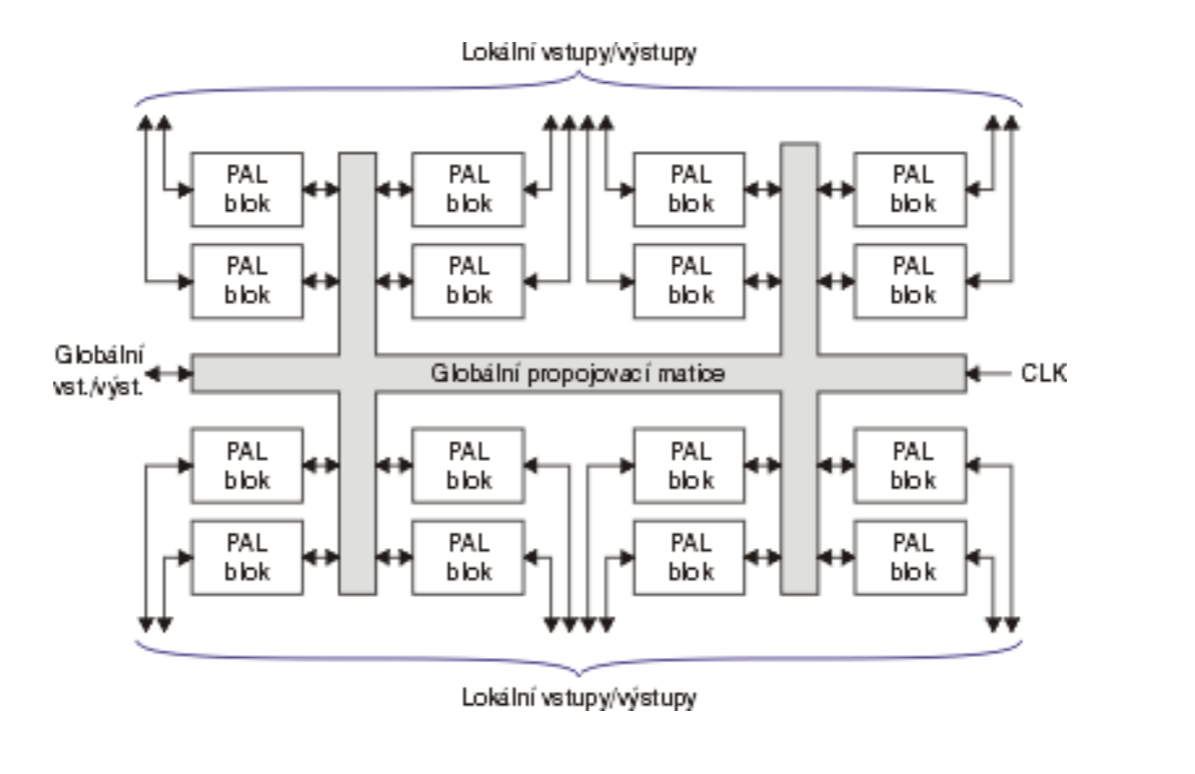
\includegraphics[scale=0.2]{sections/3_pld_npld/images/Screenshot 2024-08-22 173733.png}
\end{figure}

\vspace{25mm}

\paragraph{FPGA}
Jinou alternativou jsou obvody FPGA (on Field Programmable Gate Arrays – programovatelná hradlová pole). Od CPLD se liší tím, že po zapnutí napájení musí být jejich konfigurace vždy znovu nahrána například z paměti EEPROM nebo FLASH. Pokud je tato paměť jejich součástí, programují se po zapájení podobně jako složitější CPLD. Větší FPGA většinou neobsahují paměť EEPROM/FLASH a po zapnutí napájení je nutné je vždy znovu nakonfigurovat (takže jejich funkce na rozdíl od CPLD není okamžitě dostupná).

\begin{figure}[h]
    \centering
    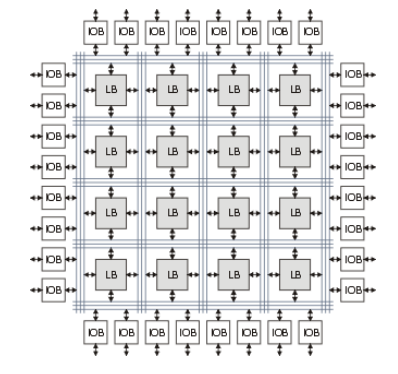
\includegraphics[scale=0.5]{sections/3_pld_npld/images/Screenshot 2024-08-22 173804.png}
\end{figure}

Velké programovatelné logické obvody dnes umožňují i implementaci komplikovaných procesorů.

\subsubsection{Makrobuňka vs logický blok}
Makrobuňka a logický blok jsou dva různé koncepty používané v programovatelných logických zařízeních (PLD), jako jsou FPGA a CPLD. Hlavní rozdíl spočívá v tom, že makrobuňky jsou typické pro CPLD a jsou jednodušší, zatímco logické bloky jsou typické pro FPGA a nabízejí vyšší flexibilitu a výkonnost.

\paragraph{Makrobuňka}
Makrobuňka je relativně malá. Je základní stavební jednotkou v CPLD. Obsahuje kombinatorické a sekvenční logické prvky, jako například AND a OR brány pro kombinatorickou logiku. Flip-flopy pro sekvenční logiku. Je schopna realizovat jednoduché logické funkce a může být nakonfigurována pro různé kombinatorické a sekvenční operace. Některé makrobuňky mohou zahrnovat také registry a multiplexery. Používají se hlavně v CPLD, kde se makrobuňky propojují pomocí pevně daných spojovacích cest.
\paragraph{Logický blok}
Logický blok je základní stavební jednotka v FPGA. Skládá se z LUT (Look-Up Table) pro implementaci kombinatorické logiky. Flip-flopů nebo registrů pro implementaci sekvenční logiky. Multiplexerů a dalších pomocných obvodů. Logický blok je více flexibilní a výkonnější než makrobuňka. LUT umožňuje realizovat libovolnou logickou funkci dané šířky (např. 4-vstupovou LUT může realizovat jakoukoliv 4-vstupovou logickou funkci).
\subsection{NPLD}
Integrované obvody, které mají pevně danou funkci již od výroby.

\subsubsection{Příklady}
\paragraph{74`164}
IC 74164 je 8-bitový sériově-paralelní posuvný registr. Má 8-bitový sériový vstup a 8 paralelních výstupů. Clk přesune data o 1 bit s každým hodinovým signálem. Clear umožňuje mazání registru.
\paragraph{74`166}
IC 74166 je 8-bitový univerzální posuvný registr, který může pracovat jak v sériovém, tak i v paralelním módu. 8-bitový sériový vstup/výstup.8-bitový paralelní vstup/výstup. Synchronní a asynchronní reset. Synchronní načítání dat. Shift/Load umožňuje volbu mezi sériovým posuvem dat a paralelním načítáním dat.
\begin{figure}[htbp]
\centering
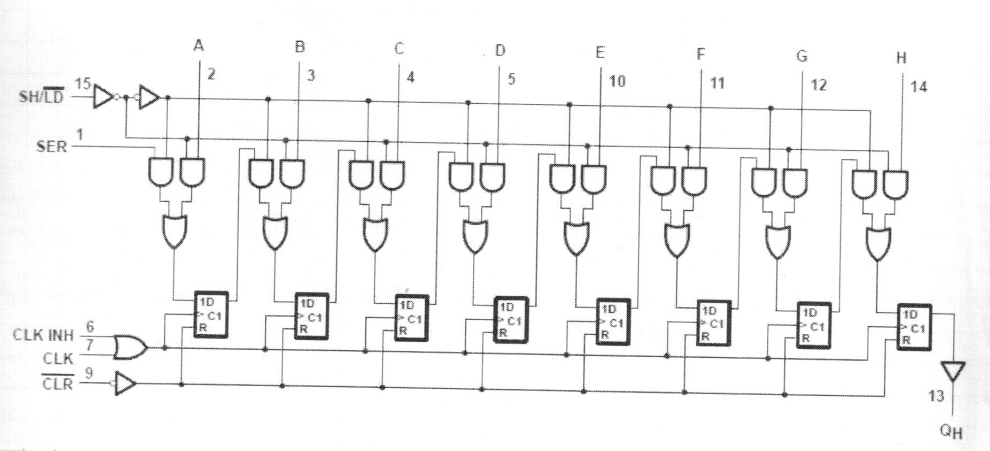
\includegraphics[scale=0.4]{sections/3_pld_npld/images/74166.png}
\end{figure}
\paragraph{74`595}
IC 74595 je známý jako 8-bitový sériově-paralelní posuvný registr s úložným registrem (latch). 8-bitový sériový vstup. 8-bitový paralelní výstup. Paměťový registr (latch). Možnost řetězení více registrů. 3 stavový výstup.
\begin{figure}[htbp]
\centering
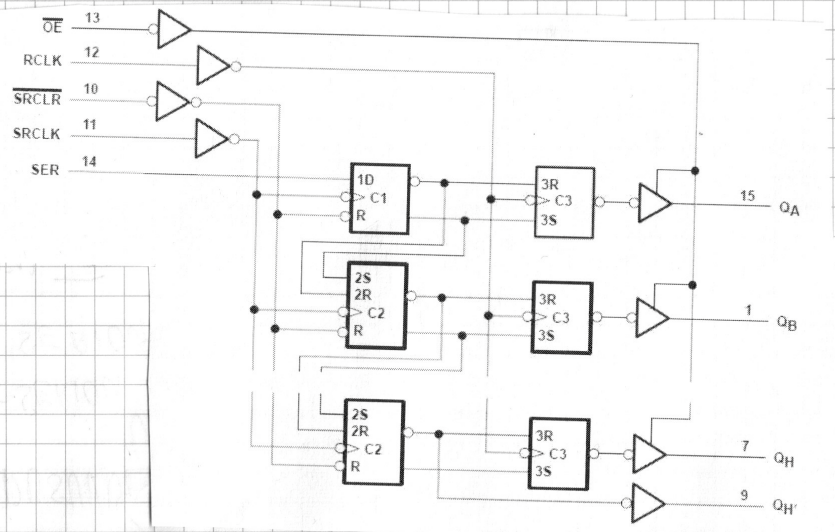
\includegraphics[scale=0.3]{sections/3_pld_npld/images/74595.png}
\end{figure}
\paragraph{74`573}
IC 74573 je 8-bitový D-type latch s třístavovým výstupem, což znamená, že má osm bitů pro ukládání dat a třístavový výstup, který může být povolen nebo zakázán.
\begin{figure}[h]
\centering
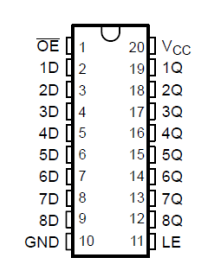
\includegraphics[scale=0.5]{sections/3_pld_npld/images/74573.png}
\end{figure}
\newpage
\paragraph{74`244}
IC 74244 je 8-bitový třístavový line driver (buffer), který se používá pro posílení signálů a ochranu datových sběrnic před nadměrným zatížením. Tento obvod je navržen tak, aby posílil digitální signály a umožnil jejich řízení na společné sběrnici s minimálním zkreslením. Dva samostatné 4-bitové ovladače, každý ovladač má vlastní enable pin. Jednosměrný.
\begin{figure}[h]
\centering
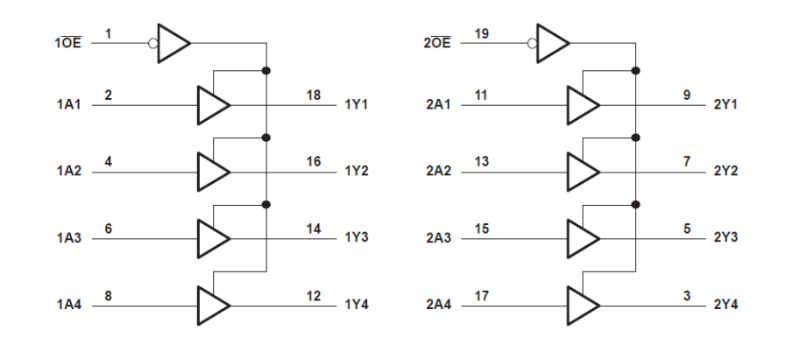
\includegraphics[scale=0.8]{sections/3_pld_npld/images/74244.png}
\end{figure}
\paragraph{74`245}
IC 74245 je 8-bitový obousměrný třístavový buffer, který se často používá v digitálních systémech pro řízení a posílení signálů na sběrnici. Tento obvod umožňuje obousměrný přenos dat mezi dvěma částmi systému.
\begin{figure}[htbp]
\centering
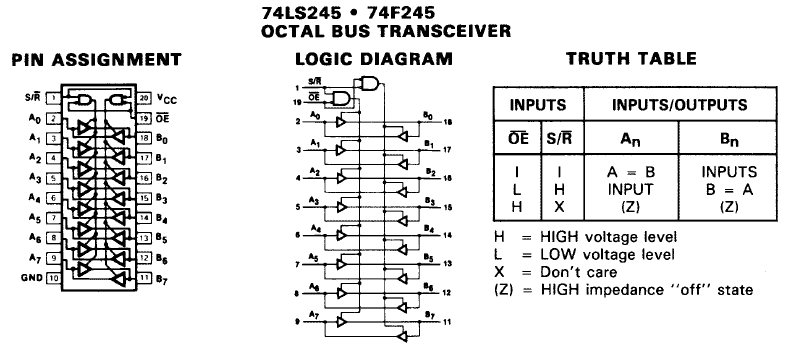
\includegraphics[scale=0.4]{sections/3_pld_npld/images/74245.png}
\end{figure}
\paragraph{74`688}
IC 74688 je 8-bitový ekvivalentní komparátor, který se používá pro porovnání dvou 8-bitových binárních hodnot. Tento komparátor je schopen generovat výstupní signály indikující, zda jsou dvě vstupní hodnoty stejné. Možnost kaskádování: umožňuje propojení více komparátorů pro porovnání delších bitových řetězců.
\begin{figure}[htbp]
\centering
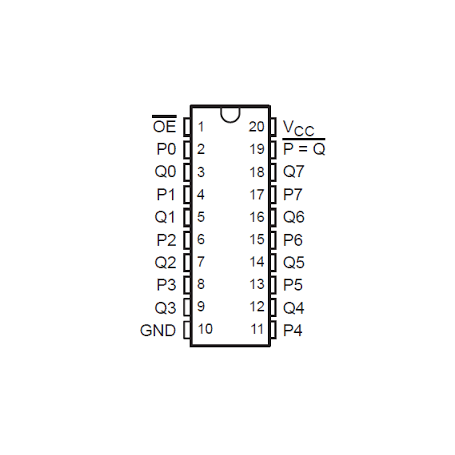
\includegraphics[scale=0.3]{sections/3_pld_npld/images/74688.png}
\end{figure}
\paragraph{74`193}
IC 74193 je 4-bitový synchronní čítač, který může provádět jak sčítání (počítání nahoru), tak odečítání (počítání dolů). Může být inicializován na libovolnou hodnotu pomocí paralelních vstupů. Carry-out a borrow-out výstupní signály pro řetězení více čítačů.
\begin{figure}[htbp]
\centering
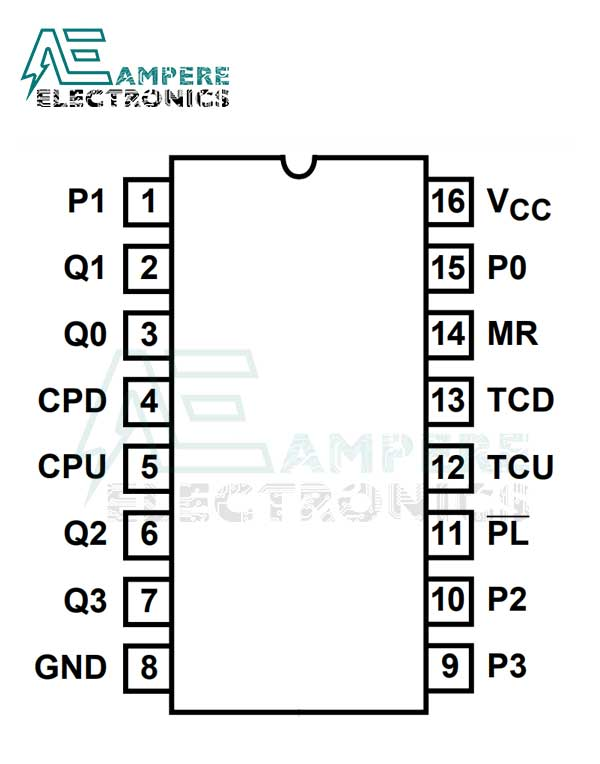
\includegraphics[scale=0.2]{sections/3_pld_npld/images/74193.jpg}
\end{figure}


